\documentclass[tikz,border=12pt]{standalone}
\usepackage[T1]{fontenc}
\usepackage{mathpazo}
\usepackage{amsmath,amssymb}
\usetikzlibrary{arrows.meta, calc, decorations.pathreplacing}

\definecolor{stblue}{HTML}{7B97AD}
\definecolor{rwgold}{HTML}{B8995E}
\definecolor{sage}{HTML}{7A9A7E}
\definecolor{dkbrown}{HTML}{3D3530}
\definecolor{wmgray}{HTML}{7B7067}
\definecolor{cream}{HTML}{F9F6F0}
\definecolor{border}{HTML}{D4C9B8}
\definecolor{terracotta}{HTML}{C47A6A}
\definecolor{lavender}{HTML}{907EA0}

\begin{document}
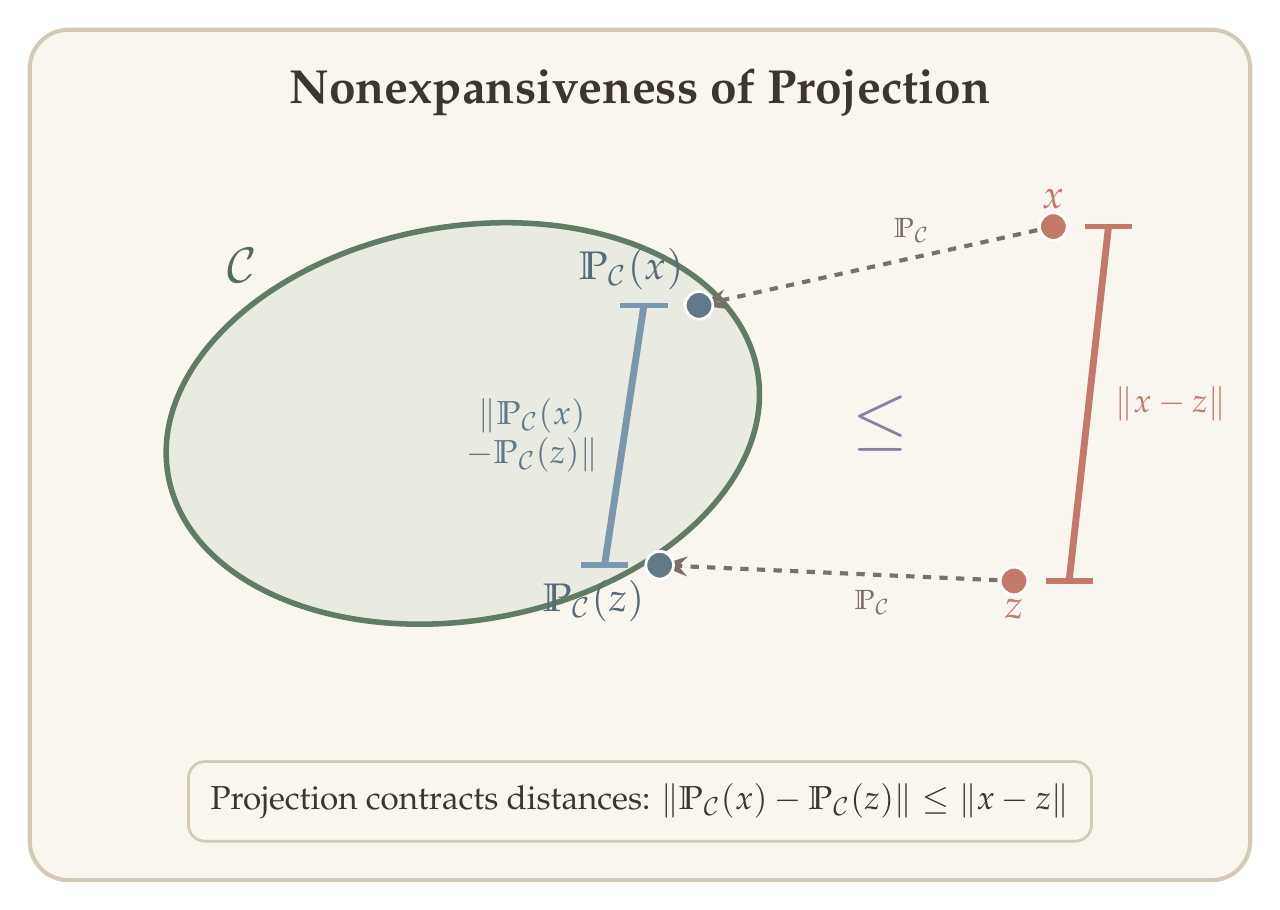
\begin{tikzpicture}[>={Stealth[length=3.5mm, width=2.5mm]}]

% Background
\fill[cream, rounded corners=14pt] (-1.5,-2.8) rectangle (14.0,8.0);
\draw[border, line width=1.5pt, rounded corners=14pt] (-1.5,-2.8) rectangle (14.0,8.0);

% Title
\node[text=dkbrown, font=\LARGE\bfseries] at (6.25,7.2)
  {Nonexpansiveness of Projection};

% Convex set C (tilted ellipse)
\begin{scope}[rotate around={10:(4.0,3.0)}]
  \fill[sage, opacity=0.12] (4.0,3.0) ellipse (3.8cm and 2.5cm);
  \draw[sage!80!black, line width=2pt] (4.0,3.0) ellipse (3.8cm and 2.5cm);
\end{scope}

% Label C
\node[text=sage!70!black, font=\LARGE\bfseries] at (1.2,5.0) {$\mathcal{C}$};

% --- Key points ---
\coordinate (x) at (11.5,5.5);       % x outside C (upper right)
\coordinate (z) at (11.0,1.0);       % z outside C (lower right)
\coordinate (Px) at (7.0,4.5);       % P_C(x) on boundary
\coordinate (Pz) at (6.5,1.2);       % P_C(z) on boundary

% --- Projection arrows (dashed) ---
\draw[wmgray, line width=1.5pt, dashed, ->]
  (x) -- (Px);
\node[text=wmgray, font=\normalsize, above=2pt]
  at ($(x)!0.4!(Px)$) {$\mathbb{P}_{\mathcal{C}}$};

\draw[wmgray, line width=1.5pt, dashed, ->]
  (z) -- (Pz);
\node[text=wmgray, font=\normalsize, below=2pt]
  at ($(z)!0.4!(Pz)$) {$\mathbb{P}_{\mathcal{C}}$};

% --- Distance between x and z (right side, vertical brace) ---
\draw[terracotta, line width=2.5pt]
  ($(x)+(0.7,0)$) -- ($(z)+(0.7,0)$);
% Tick marks at ends
\draw[terracotta, line width=2pt]
  ($(x)+(0.4,0)$) -- ($(x)+(1.0,0)$);
\draw[terracotta, line width=2pt]
  ($(z)+(0.4,0)$) -- ($(z)+(1.0,0)$);
\node[text=terracotta, font=\large\bfseries, right=6pt]
  at ($(x)!0.5!(z)+(0.7,0)$) {$\|x - z\|$};

% --- Distance between P(x) and P(z) (left of projections) ---
\draw[stblue, line width=2.5pt]
  ($(Px)+(-0.7,0)$) -- ($(Pz)+(-0.7,0)$);
% Tick marks
\draw[stblue, line width=2pt]
  ($(Px)+(-0.4,0)$) -- ($(Px)+(-1.0,0)$);
\draw[stblue, line width=2pt]
  ($(Pz)+(-0.4,0)$) -- ($(Pz)+(-1.0,0)$);
\node[text=stblue!80!black, font=\large\bfseries, left=6pt, align=center]
  at ($(Px)!0.5!(Pz)+(-0.7,0)$) {$\|\mathbb{P}_{\mathcal{C}}(x)$\\$- \mathbb{P}_{\mathcal{C}}(z)\|$};

% --- Inequality symbol ---
\node[text=lavender, font=\Huge\bfseries] at (9.3,3.0) {$\leq$};

% --- Points (on top) ---
\fill[terracotta] (x) circle (5pt);
\draw[white, line width=1pt] (x) circle (5pt);
\node[text=terracotta, font=\Large\bfseries, above=3pt] at (x) {$x$};

\fill[terracotta] (z) circle (5pt);
\draw[white, line width=1pt] (z) circle (5pt);
\node[text=terracotta, font=\Large\bfseries, below=3pt] at (z) {$z$};

\fill[stblue!80!black] (Px) circle (5pt);
\draw[white, line width=1pt] (Px) circle (5pt);
\node[text=stblue!70!black, font=\Large\bfseries, above left=2pt] at (Px)
  {$\mathbb{P}_{\mathcal{C}}(x)$};

\fill[stblue!80!black] (Pz) circle (5pt);
\draw[white, line width=1pt] (Pz) circle (5pt);
\node[text=stblue!70!black, font=\Large\bfseries, below left=2pt] at (Pz)
  {$\mathbb{P}_{\mathcal{C}}(z)$};

% --- Annotation box (using node with draw, avoids separate fill/draw/text) ---
\node[text=dkbrown, font=\large,
      fill=cream, inner sep=8pt,
      draw=border, line width=1pt, rounded corners=6pt]
  at (6.25,-1.8)
  {Projection contracts distances:
   $\|\mathbb{P}_{\mathcal{C}}(x) - \mathbb{P}_{\mathcal{C}}(z)\| \leq \|x - z\|$};

\end{tikzpicture}
\end{document}
